\chapter{Geospatial Data on the Web}
\label{ch:ch1}

\begin{itemize}
\item Traditional GIS data
\item soA on vocabularies
\item soA of geo support in triple stores
\item Contributions
\item conclusion
\end{itemize}


\section{Traditional Geospatial Data}
   \subsection{Specifities}
   \subsection{Formats}

\section{Vocabularies for Geospatial Data}
\textcolor{red}{Add here the studies of Atemezing:TC12 }

\section{Georeferencing data on the Web}
\label{sec:georef}
Georeferencing data either by direct or indirect spatial reference requires some reference datasets that can be used as the spatial frame for anchoring these thematic data. Especially, it requires data on both CRSs and named places, which must be published on the Web of data.

\subsection{Identifying and describing CRSs on the Web}
In order to fulfill the need for CRS identification and description on the Web, OGC maintains a set of URIs for identifying the most commonly used CRS. While very useful, the main disadvantage of this proposal is that the URIs defined by OGC are not very intuitive for users who are not familiar with Spatial Reference System Identifiers defined by geographic information authorities like OGC or EPSG, such as ``4326'' (which actually refers to a WGS84 CRS defined by the EPSG). Moreover, many CRS commonly used locally, such as deprecated French projected CRS, are not available in that registry. In addition to OGC proposal, several registries have been proposed by the geographic information community for cataloguing existing CRSs.
The EPSG Geodetic Parameter Registry\footnote{\url{http://www.epsg-registry.org/}} allows querying the Geodetic Parameter Dataset gathered by the EPSG. CRSs can be retrieved by name, by code, by type or by coverage area, and their characteristics are displayed on a HTML form. Unfortunately, there is no direct access to these data through dereferenceable URIs.

\subsection{Direct georeferencing of data on the Web}
\label{sec:directgeo}
Modeling direct location information such as coordinates or vector data geometries in RDF still poses some challenges. \textcolor{red}{In~\cite{Atemezing:TC12}}, we have conducted a survey of the vocabularies used for representing geographical features from vocabularies of feature types to vocabularies for geometric primitives which provide ways for representing extents, shapes and boundaries of those features. 
Most of vocabularies dedicated to geometry representation reuse W3C Geo vocabulary which allows only WGS84 coordinates, such as NeoGeo\footnote{\url{http://geovocab.org/doc/neogeo/}}. With the rise of the Open Data movement, more and more publishers including governments and local authorities are releasing legacy data that are georeferenced using others CRSs. For example, IGN France releases data using different projected CRSs depending on the geographic extent of each dataset. In order to overcome this limitation on CRSs, the vocabulary designed by OGC GeoSPARQL standard  does not reuse W3C Geo vocabulary but proposes another class ``Point'' instead. Geometries of geographical data represented in RDF with the GeoSPARQL vocabulary are represented by literals encoded consistently with other OGC standards. \texttt{gsp:wktLiteral} and \texttt{gsp:gmlLiteral} are thus respectively derived from Well-Known Text and GML encoding rules. In \texttt{wktLiteral} and \texttt{gmlLiteral}, the CRS used to define the coordinates of the point is identified by a dereferenceable URI which is explicitly stated at the beginning of the literal. This way of associating coordinate reference systems with geometries has the advantage of being consistent with Linked Data principles: each CRS is identified with a dereferenceable URI. The main drawback is that such literals cannot be easily queried with SPARQL, unless using regular expression-based filters.  To overcome this limitation, we propose in the geometry vocabulary presented in \textcolor{red}{Section 3} to associate each geometry to the CRS used by its coordinates with the property \texttt{geom:crs}.

\subsection{Indirect georeferencing of data on the Web}
\label{sec:indirectgeo}
Modeling indirect location information such as administrative units or named points of interest in RDF is preferably done by identifying such geographic features with URIs and describing them by their properties, so that they can be referenced by other datasets. This is the case in one of the most reused datasets of the Web of data, namely Geonames\footnote{\url{http://sws.geonames.org/}}. However, there are yet very few reference datasets for the French territory on the Web of data.  A simple example is the current resource for \textit{Paris} in the French DBpedia\footnote{\url{http://fr.dbpedia.org/resource/Paris}}. The department's name associated to this resource is a literal named ``Paris'' and the different arrondissements composing the city are modeled as \texttt{skos:Concept} instead of \texttt{dbpedia-owl:Place}. Even Geonames data remain very limited, as French administrative units are provided as simple geometries (POINT). The ``Official Geographic Code''\footnote{\url{http://rdf.insee.fr/sparql}} published by the French Statistical Institute (INSEE) is the most up-to-date and accurate dataset on French administrative units, but unfortunately it contains no geometrical description of their boundaries. This has the consequence of not having a baseline during mapping process for application developers trying to consume specific data coming from France. Datasets describing administrative units, points of interest or postal addresses with their labels and geometries, and identifying these features with URIs could be used with benefits not only for georeferencing other datasets, but also for interlinking datasets georeferenced by direct and indirect location information.


\section{Contributions}

\textcolor{red}{Describe the contributions on geometry and geography vocabularies. Reuse mainly the recent work to be presented at Terra Cognita 2014}

\subsection{Vocabularies for Geometries and Feature Types} \label{sec:topovocab}

Direct georeferencing of data implies representing coordinates or geometries and associating them to a CRS.  This requires vocabularies for geometries and CRSs. Besides, indirect georeferencing of data implies associating them to other data on named places. Preferably, these data on named places should be also georeferenced by coordinates in order to serve as basis for data linking between indirectly and directly georeferenced datasets. In this section, we present the vocabularies that we have defined and reused for geographic data publishing.
This requires reference geographic data on named places and therefore vocabularies for describing feature types and their properties. 

\subsubsection{A vocabulary for geometries} \label{sec:geomvocab}
In~\cite{Atemezing:TC12}, we already surveyed numerous vocabularies for representing geographical features and their geometries, either using a literal (e.g. wktLiteral) or a structured representation \`a la NeoGeo. We concluded the survey with some recommendations for geometry descriptions:
\begin{itemize}
 \item the distinction of geometry versus feature and a property linking both classes (e.g. for attaching provenance information on how some points of a geometry have been collected),
 \item the ability to represent structured geometries (e.g. for performing simple spatial queries on the data, even when they are stored in a triple store that do not implement the GeoSPARQL standard),
 \item the integration of any coordinate reference system  (e.g. for allowing projected coordinates for cartographic purposes).
\end{itemize}
In addition to these recommendations, we also think that the domain of the property used to link a feature to its geometry should be left empty in order to accept links between any type of resource and a geometry. This would be useful for example, to associate a person to the coordinates of their birthplace.


\subsubsection{Extending GeoSPARQL vocabulary}
In order to fulfill these recommendations, we have developed a new vocabulary that re-uses and extends the existing vocabularies for representing geometries, namely:
\begin{itemize}
 \item \url{http://www.opengis.net/ont/geosparql#} (prefix \texttt{gsp}). This vocabulary provides the basic concepts to represent geographical data such as SpatialObject, Feature or \texttt{Geometry}. A Feature is linked to a Geometry via the relation \texttt{gsp:hasGeometry}. The geometries are typed strings (\texttt{gsp:gmlLiteral} or \texttt{gsp:wktLiteral} corresponding respectively to the properties \texttt{gsp:asGML} and \texttt{gsp:asWKT}). The vocabulary contains also spatial functions.
 \item \url{http://www.opengis.net/ont/sf#} (prefix \texttt{sf}): This vocabulary is based on the OGC standard Simple Features Access \cite{iso2004}. The class \texttt{sf:Geometry} is a subclass of \texttt{gsp:Geometry}. 
\end{itemize}
 
Reusing and extending GeoSPARQL Simple Features vocabulary with structured geometries  \`a la NeoGeo enables us to represent geometries both with GeoSPARQL compliant literals and with structured geometries that can be handled easily with SPARQL. The extension for structured geometries consists in defining a subclass for each class from the \texttt{sf} vocabulary, and defining properties to associate its instances with a CRS and coordinates or other suitable geometric primitives. For example, the class \texttt{geom:Point} is a subclass of \texttt{sf:Point}. An instance of \texttt{geom:Point} is associated with exactly one instance of \texttt{ignf:CRS} via the property \texttt{geom:crs}, and it
has exactly one coordinate X and exactly one coordinate Y. It can also have a Z coordinate. The coordinates are \texttt{xsd:double} and correspond to the properties \texttt{geom:coordX:}, \texttt{geom:coordY:} and \texttt{geom:coordZ:} respectively. Other complex geometries are also defined, such as Linestrings, LinearRings, Polygons or MultiPolygons. Their definitions are based on the class \texttt{geom:Point}. As an example, an instance of \texttt{geom:Linestring} is defined as an instance of \texttt{geom:PointsList} which is an ordered \texttt{rdf:List} of instances of \texttt{geom:Point} designated by the property \texttt{geom:points}.


We have also defined a property \texttt{geom:geometry} with an empty domain. Thus, our proposal defines a more generic class for a \textsf{POINT} with the benefit of choosing the CRS of the underlying data. Figure \ref{fig:geomcrs} gives an overview of the relationships between the high level concepts with geometries, CRS and topographic features.

\begin{figure}[!htbp]
\vspace{-13pt}
  \begin{center}
  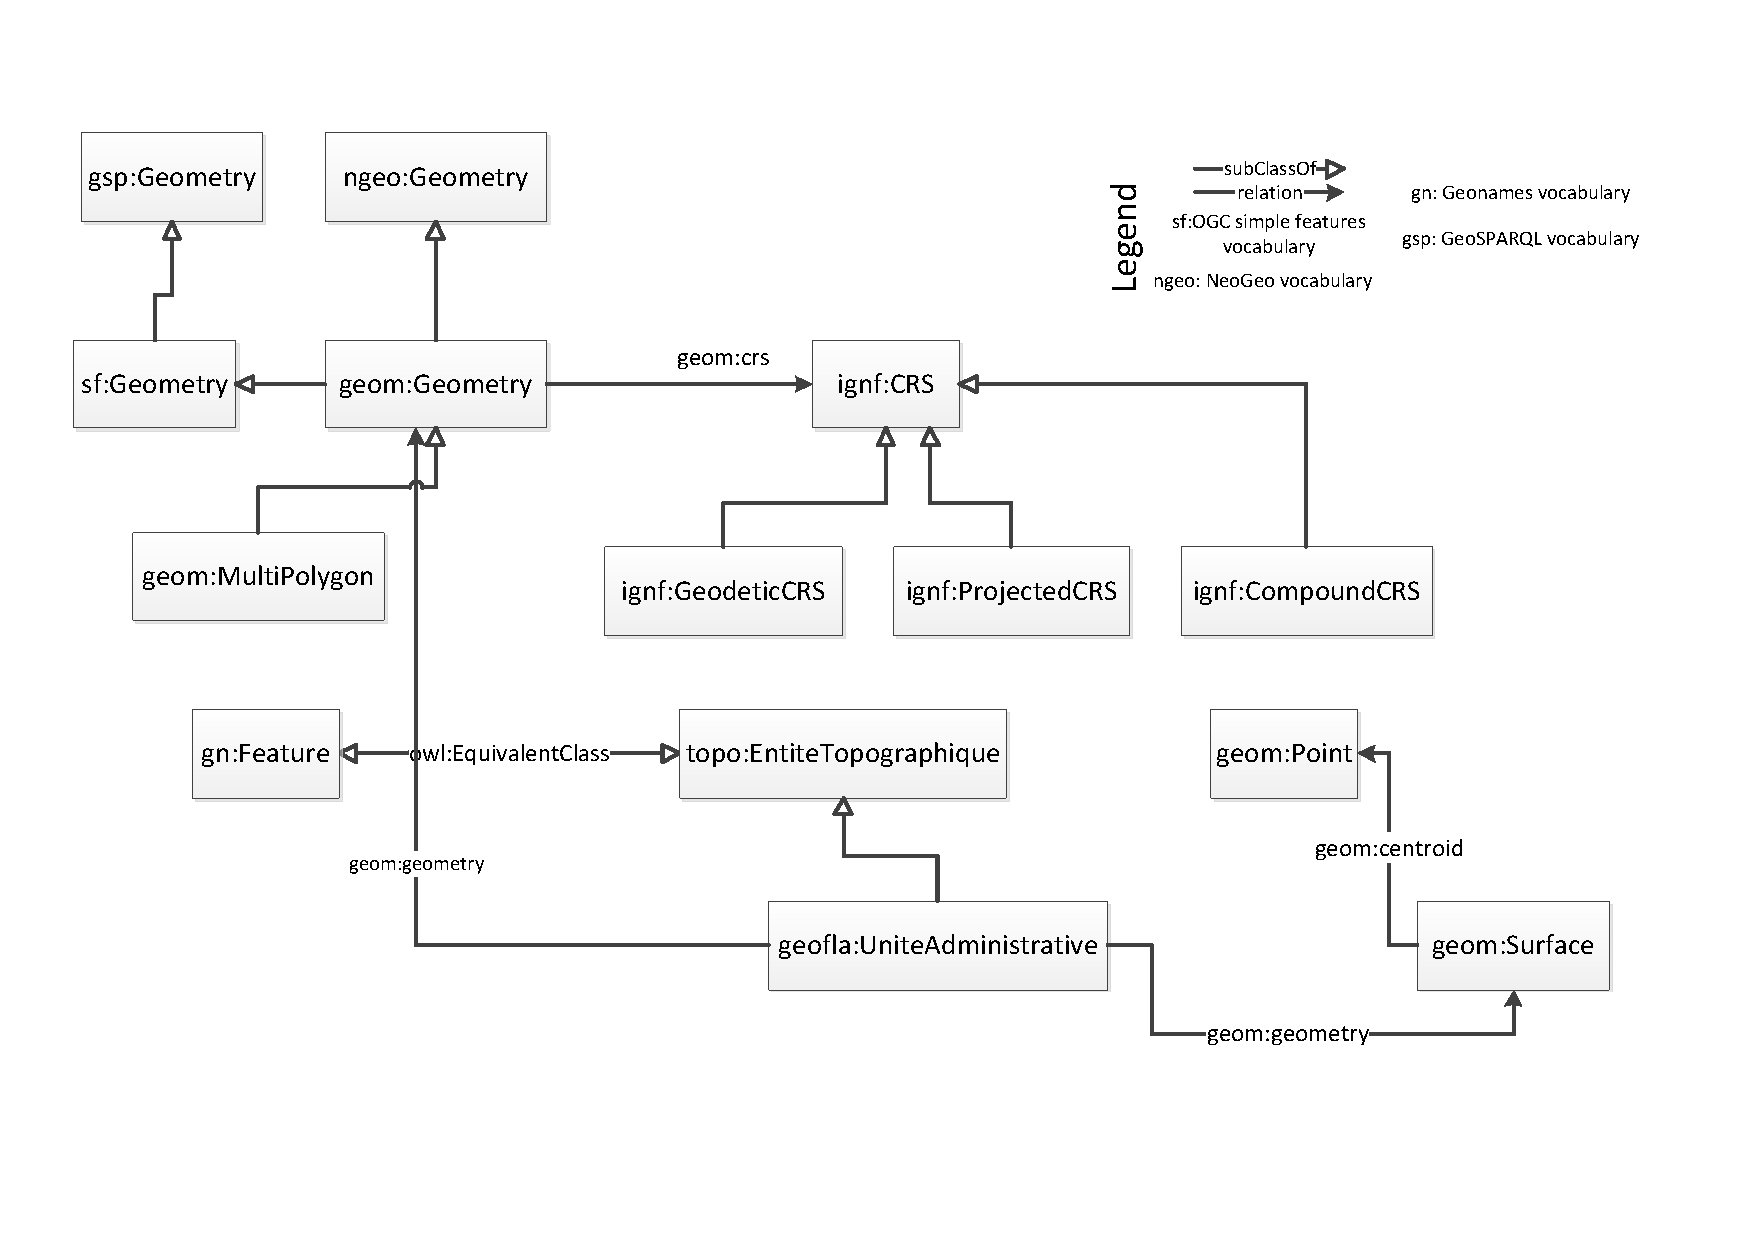
\includegraphics[width=0.8\textwidth]{img/vocabs-ign.pdf}
  \vspace{-15pt}
  \caption{High level classes of ignf, geom and topo vocabularies; relationships between them and mappings with external vocabularies.}
  \vspace{-10pt}
  \label{fig:geomcrs}
  \end{center}
\end{figure}



\subsection{CRS requirements for the  French territory} \label{sec:reqs}

As explained in Section \ref{sec:context}, making explicit the CRS used in a given dataset is a very important issue when dealing with direct location data. This is especially important in the field of geographical information where different CRSs are commonly used due to technical or legal requirements. For INSPIRE Directive, CRS are considered as reference data used for linking thematic data \cite{inspire2009}, and must be described according to ISO 19111 standard. To be consistent with Linked Data principles, CRS should be identified by URIs, like in OGC proposal. Moreover, as Linked Data users are not always familiar with CRS identifiers commonly used within the geographic information community, URI used to identify CRS should use more intuitive names. Finally, consistently with our goal of contributing to a better georeferencing of data on the French territory, we need an access to the descriptions of all French CRSs, including some deprecated but still used CRSs like ``Lambert 1''.



\begin{table}[!htp]
\centering{
\begin{tabular}{lr}
\specialrule{1pt}{1pt}{1pt}
 \textbf{Prefix}	& 	\textbf{URI}	  \\ \specialrule{1pt}{1pt}{1pt}
geofla 	   & \url{http://data.ign.fr/def/geofla#}  \\
geom &  \url{http://data.ign.fr/def/geometrie#} \\
ignf &  \url{http://data.ign.fr/def/ignf#} \\
rgeofla &  \url{http://data.ign.fr/id/geofla/} \\
topo &  \url{http://data.ign.fr/def/topo#} \\
rtopo &  \url{http://data.ign.fr/id/topo/} 

		\\ \specialrule{1pt}{1pt}{1pt}
\end{tabular}
\caption{ URI schemes and conventions used for vocabularies and resources.}
\label{tab:uris}
}
\end{table}

The Information and Service System for European Coordinate Reference Systems\footnote{\url{http://www.crs-geo.eu}}  provides an access to ISO 19111 standard-based descriptions of the main European CRSs but has the same limitation as the EPSG registry: access to the descriptions is not allowed by URI, but only through a cartographic interface.
\url{SpatialReference.org} initiative aims at allowing users to use URI-based references to spatial reference systems, including some CRSs defined and maintained by IGN France.  Besides, the proposed URL policy is not very intuitive. As an example, this URL identifies the projected system defined by IGN France, Lambert 93: \url{http://spatialreference.org/ref/sr-org/7527/}. Moreover, the definitions of some deprecated CRSs such as Lambert zone projected CRSs (which are still used in some datasets) seem to be referenced only for the authority EPSG and not for IGNF, which also maintains a registry of CRSs. ISO 19111 standard-based definitions of all CRSs defined and maintained by IGN France are  published in an XML file\footnote{\url{ http://librairies.ign.fr/geoportail/resources/IGNF.xml}}.
References to equivalent definitions provided by the EPSG registry are explicitly stated with EPSG SRID. CRSs are identified by URIs using short names instead of numeric codes. For example, \url{http://registre.ign.fr/ign/IGNF/crs/NTFLAMB2E}  is the URI designed for the ``Lambert 2 \'{e}tendu'' projected system. Indeed ``NTFLAMB2E'' is used to identify the projected system ``Lambert 2 \'{e}tendu'' which is based on NTF (New French Triangulation) geodetic reference system. Unfortunately, this registry is still in evolution and its URIs are not dereferenceable yet.
 
%\paragraph{Publishing a dataset on French CRSs}
As no existing registry fulfilled all our requirements, we have developed a vocabulary\footnote{\url{http://data.ign.fr/def/ignf}}, inspired from the ISO 19111 schema for CRSs description. Then we have converted IGNF CRSs registry into RDF, and published this dataset on the Web with the Datalift platform\footnote{A service to lookup CRS in RDF can be found at \url{http://www.eurecom.fr/~atemezin/ignf-lookup/}}. Therefore, the description of the ``NTF Lambert 2 \'{e}tendu'' projected CRS can be retrieved at this URL \url{http://data.ign.fr/id/ignf/crs/NTFLAMB2E}.

\subsection{Vocabularies for Geographic Feature Types}
\label{sec:vocgeofeature}

Indirect georeferencing of resources on the Web requires reference geographic data on named places and therefore vocabularies for describing feature types and their properties. Therefore, we have chosen to publish a reference dataset on administrative units called GEOFLA\circledR, which is already available in GIS format under an Open Data license. We have also made tests of data conversion and interlinking with another largest dataset on French names places. We have produced and published two vocabularies to describe these datasets, to make sure that all concepts and properties needed would be available.
In the GEOFLA\circledR ~vocabulary, 5 classes have been defined: commune, canton, arrondissement, department and region. In the BD TOPO\circledR ~vocabulary\footnote{\url{http://data.ign.fr/def/topo}} $35$ main classes have been defined. They represent the main types of geographic features represented in the BD TOPO\circledR ~database. In both vocabularies, properties have been defined based on the attributes of their related classes in the databases. The geographic feature types defined as values of attributes ``nature'' are modeled as instances of \texttt{skos:Concept}. SKOS is intensively used to easily group concepts into different schemes (using \texttt{skos:hasTopConcept}) and provide semantic relationships (e.g: \texttt{skos:broader}, \texttt{skos:narrowMatch}) among them. We also provide alignments with Geonames vocabulary, where \texttt{topo:Place} is subclass of \texttt{gn:S} and \texttt{owl:sameAs} linked concepts.\footnote{\url{https://github.com/gatemezing/ign-iswc2014/blob/master/vocabularies/mappingsGeonames.ttl}} 

All the classes are defined as subclasses of  \texttt{topo:EntiteTopographique} which defines the representation of a real world entity associated to a location relative to the Earth, consistently with ISO TC 211 and OGC standards. 
The GEOFLA\circledR 's application schema is composed of classes representing different types of french administrative units, namely communes, cantons, arrondissements and departments. In \texttt{geofla} vocabulary, we add a class region  from the instances of the class department via two attributes  that precise to what region each instance of department belongs.  Their properties are defined based on the attributes of their related classes in GEOFLA\circledR ~database.

Regarding use cases consuming  real-world databases developed using the vocabularies aforementioned, two different applications have been developed. namely \textit{PerfectSchool}\footnote{\url{semantics.eurecom.fr/datalift/PerfectSchool/}}  and \textit{Equipment}\footnote{\url{http://semantics.eurecom.fr/datalift/Equipment/}}. The former is a mobile application intended to provide useful information on schools in France, while the latter is a facet view by categories of facilities in France, specifically in the city of Toulouse. 
A Commune has an attribute called \textit{``nature''} whose enumerated values precise whether the commune is the capital of a bigger administrative unit, modeled in the vocabulary by the ObjectProperty \texttt{geofla:statut} with range \texttt{skos:Concept} defined in this specific \texttt{skos:ConceptScheme} \url{http://{BASE}/codes/geofla/typedecommune/liste} pointing to the different types of French administrative unit's capital. 

\textcolor{red}{
\subsection{Publishing structured geometries from geographic data}
The vocabulary for geometry reused by a geodata converter that takes traditional GIS data as input and outputs RDF data with geometries defined both with a \texttt{gsp:wktLiteral} and with a structured representation compliant with our vocabulary. Geometries are automatically associated with the chosen CRS. This converter is implemented as a plugin of the Datalift platform and can be reused easily for geographic data publishing purpose.
}
